\documentclass[12pt]{spieman}
\usepackage{amsmath}
\usepackage{amsfonts}
\usepackage{graphicx}
\usepackage{setspace}

\setlength{\headheight}{14.0pt}
\addtolength{\topmargin}{-1.0pt}
\setlength{\footskip}{12.6pt}


\begin{document} 

\title{Lab2 Latex}

\tableofcontents
\newpage


\begin{abstract}
We present a system for finding and tracking a face and extract global and local animation parameters from a video sequence. The system uses an initial colour processing step for finding a rough estimate of the position, size, and inplane rotation of the face, followed by a refinement step drived by an active model. The latter step refines the previous estimate, and also extracts local animation parameters. The system is able to track the face and some facial features in near real-time, and can compress the result to a bitstream compliant to MPEG-4 face and body animation. 
\end{abstract}

\keywords{Active appearance tracking models; Quickly finding the location of the face; Skin color matching algorithm}


\begin{spacing}{2}   

\section{Our active model and it’s parameterization}
\label{sect:intro}  % \label{} allows reference to this section
Our active model is a simplification of the AAM, and we describe here the model and how it is parameterized. As a starting point, we use the wireframe face model Candide, which has been popular in video coding research for many years. The third variant of this model, Candide-3, is also compliant to MPEG-4 Face Animation. The Candide model has manually been adapted to a set of images by varying a set of 12 parameters
\begin{itemize}
    \sloppy
    \item the first six parameters are the global motion (or pose) parameters; 3D-rotation, 2D-translation, and scale. We denote the pose parameter vector $\pi = [r_x ,r_y ,r_z ,t_x ,t_y ,z]^T$;
    \sloppy
    \item the remaining parameters are activation levels for six action units (from FACS, the facial action coding system [2]) controlling the lips and eyebrows. They are contained in the vector $\sigma$, and control the shape of the head according to \eqref{eq1}
\end{itemize}

We collect those parameters in a 12D vector $pT = [\pi T, \sigma T]$, which parameterizes the geometry of the model. Thus, the geometry is described by

\begin{equation}
    g(p)= R(z + 1)(\bar{s}+ S\sigma)+ \tau, 
    \label{eq1}
\end{equation}
where $\sigma$ is the vector of action unit activation levels, \\
$s$ is the standard shape of the Candide model, \\
$\tau = \tau(tx,ty)$ is a function of the x- and y-translations, \\
$R = R(rx ,ry ,rz)$ is a rotation matrix created from the three rotation parameters, and z is a scaling factor.

The image under the model has, for each image in the training set, been mapped onto the model, creating a texture mapped wireframe model. The model has then been normalized to a standard shape, size, and position (i.e., $p = 0 \Rightarrow{} g = \bar{g}$), in order to collect a geometrically normalized set of textures. On this set, a PCA has been performed and the eigentextures (shape free eigenfaces, geometrically normalized eigenfaces) have been computed. 

\begin{figure}[H]
    \centering
    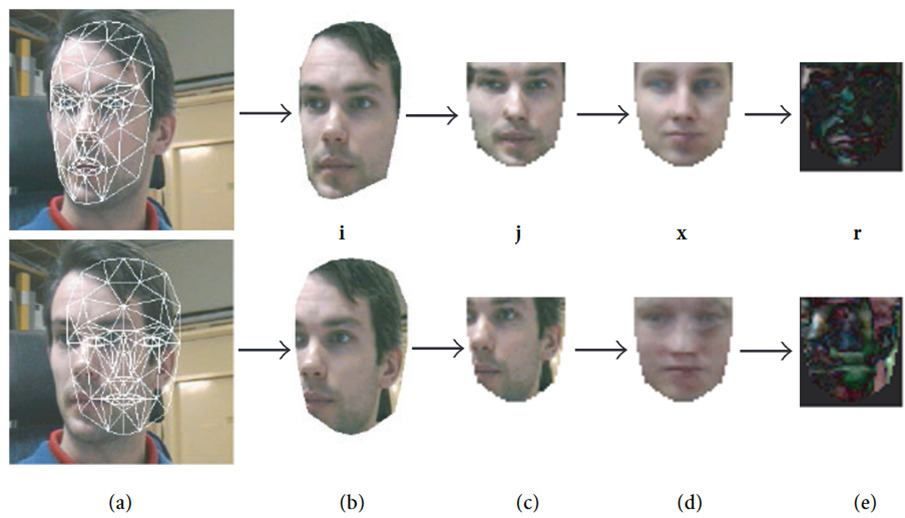
\includegraphics[width=130mm]{Figure1.jpg}
    \caption{The model matching and texture approximation process. (a) A good and a bad (top and bottom row, respectively) model adaptation is shown; (b) the image mapped onto the model; (c) the model is reshaped to the standard shape, producing the image j; (d) the normalized texture is approximated by the eigentextures, producing the image x; (e) the residual image r is computed. The better the model adaptation is, the more similar the images j and x are. Analysis of the image r tells us how to improve the model adaptation, that is, how to minimize the difference between j and x.}
    \label{fig1}
\end{figure}



\subsection{Matching the model and the image}{}As in (…) we can create the normalized input image $j(p)$. The texture parameters minimizing the model error $e(p)$ are then given by projecting the normalized input image $j(p)$ on the eigentextures, that is


\begin{equation}
    \xi = XT (j(p)- \bar{x})
\end{equation}

Thus, $p$ is the only necessary parameter in our case:

\begin{equation}
    g = g(p), x = x(p),
\end{equation}

Where

\begin{equation}
    x(p)= \bar{x}+ XXT (j(p)- \bar{x}),
\end{equation}


The entire process from input image to normalized is illustrated in Figure \ref{fig1}. Note that our model is not a complete appearance model, since we parameterize the geometry only and let the texture depend on the input image as well. For an appearance model, a PCA is performed to find the suitable subspace of appearance modes combining deformation modes and texture modes (eigentextures). In our application, we only parameterize the model in terms of deformation (including global motion) since we know in advance what kind of parameters we are interested in extracting. If we want to extract action units (the parameters typically used for Candide), we simply parameterize and train our model on those parameters (or deformations spanning the same subspace). We can still use the AAM search exactly as described above.

\subsection{Training the model}

To try out this scheme, the model has been adapted (manually in the beginning, then semiautomatically) to 330 images of six different persons from different angles and with different facial expressions. The following action units from FACS have been chosen as deformation parameters:


\begin{enumerate}
    \item Jaw drop
    \item Lip stretcher
    \item Lip corner depressor
    \item Upper lip raiser
    \item Eyebrow lowerer
    \item Outer eyebrow raiser
\end{enumerate}
The adapted model, for each image, has been normalized to a standard shape with the size 40 × 42 pixels, as in Figure 1c, top row, and a PCA has been performed on the resulting training textures to compute the eigentextures. The mean texture $\bar{x}$ and the DC-level have been subtracted from the training textures prior to the PCA. With the eigentextures available, all the parameters have been perturbed, one by one and for each image, in steps of 0.01 in the range [-0.1, 0.1], and the matrix G estimated. From G, the update matrix U has been computed.

The experiments presented here are performed on a PC with a 500 MHz Intel Pentium III processor and an ASUS V3800 graphics card with video input. The color-based algorithm runs in approximately 0.1 seconds, and the AAM search requires about 15 ms/iteration. Typically, less than 10 iterations are needed per frame, and fewer iterations are needed the


\begin{figure}[H]
    \centering
    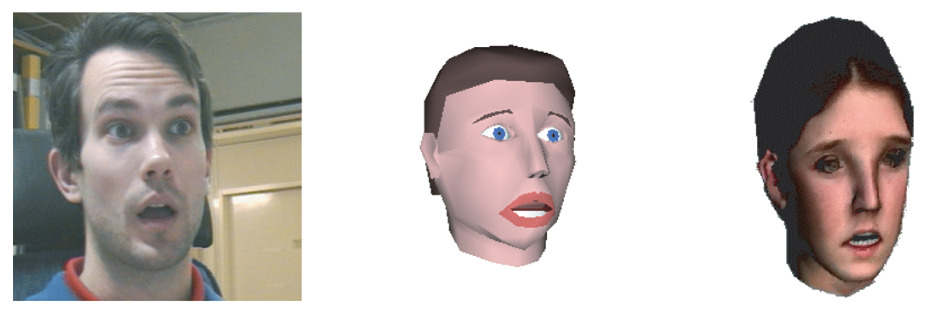
\includegraphics[width=120mm]{Figure2.jpg}
    \caption{The original frame (left), the frame synthesized with FAE from DIST, University of Genova (middle), and the facial animation system by Miralab, University of Geneva (right). The corresponding Candide model adaptation is shown in Figure 3 (right)}
    \label{fig2}
\end{figure}

\begin{table}[H]
\caption{Timing results (average over 341 frames).} 
\label{tab1}
\begin{center}       
\begin{tabular}{|l|l|l|} 
\hline
\rule[-1ex]{0pt}{3.5ex}  Measurement & RGB & Grayscale \\
\hline\hline
\rule[-1ex]{0pt}{3.5ex}  Iterations per frame & 6.9 & 6.8  \\
\hline
\rule[-1ex]{0pt}{3.5ex} time per frame (ms) & 94.1 & 69.1 \\
\hline
\rule[-1ex]{0pt}{3.5ex}  Time per iteration (ms) & 13.6 & 10.2   \\
\hline
\rule[-1ex]{0pt}{3.5ex} Time for computing $\Delta$p & 7.2 & 5.05. \\
\hline 
\end{tabular}
\end{center}
\end{table}
Closer the initial estimate is to the optimum. Thus, if a video sequence is recorded at a high frame rate (with small motion between each frame), the tracking will also run at a higher speed. Visual results are shown in Figure (…). Using grayscale eigentextures and update data, it turned out that the computation in the graphics card (which internally uses RGB) became almost 20\% slower. However, the computations performed on the CPU became (as expected) about 3 times faster, and then only 20\% of the total computing time is due to the CPU (the rest being computations in the graphics card). Testing on a video sequence of a few hundred frames gave results according to Table \ref{tab1}. It is clear that grayscale computations are preferable, since the visual results are equivalent. Snapshots from the animation of the resulting MPEG-4 Face Animation bitstream using two different facial animation systems are shown in Figure \ref{fig2}. model does not converge to a small error measure, the colour-based algorithm is invoked, handing a new initial estimate to the active model. Re-initialization issues are discussed in [21]. Fourth, our currently used set of action units is not complete. For example, we do not analyse the motion of the eyelids at all, and the shape of the head is assumed to be known a priori.

\begin{equation}
    G_{j} = \sum\limits_{k} (r(p+\Delta p_{jk})-r(p)),
    \label{eq5}
\end{equation}
where $\Delta p_{jk}$ is a vector that perturbs $p$ in the jth componentto the amount of $k$·$c$ for some suitable constant $c$.


\begin{equation}
    T^{\mu}_{t} = \frac{\sum\limits_{\upsilon=1}^{\nu} w^{\upsilon}_{t} \odot T^{\upsilon}_{t}}{\sum\limits_{\upsilon=1}^{\nu} w^{\upsilon}_{t}}
\end{equation}


\end{spacing}
\end{document}